% ------------------------------------------------------------------------------
% Visão geral de LPS's para Android
% Autores:
%     Adorilson Bezerra <adorilson@gmail.com>
% Licença Creative Commons Atribuição 3.0. 
% Você pode usar e alterar este documento, 
% mas deve obrigatoriamente citar a autoria. 
% ------------------------------------------------------------------------------

\documentclass[a4paper,12pt]{report}

% ------------------------------------------------------------------------------
\usepackage[top=3cm,left=3cm,right=2cm,bottom=2cm]{geometry}
\usepackage[utf8]{inputenc}
\usepackage[brazil]{babel}
\usepackage[pdftex]{graphicx}
\usepackage[normalem]{ulem}   % Sublinhar textos
\usepackage{pslatex}          % Usa fontes standard ao invés das fontes do
                              % LaTeX, melhorando a qualidade dos pdfs gerados
% ------------------------------------------------------------------------------

\title
{
    \vspace{1.5cm}
    \begin{table}[h]
    \centering
    \setlength{\arrayrulewidth}{3.5\arrayrulewidth}
        \begin{tabular}{c}
        \hline\\
        \vspace{0.3cm}\Huge Visão geral de LPS's para Android\\
        \hline
        \end{tabular}
    \end{table}
}
\author
{
    Adorilson Bezerra\\
    \{adorilson@gmail.com\}
}
\date{\vspace{1.5cm}\today}

% ------------------------------------------------------------------------------
\begin{document}

\maketitle

\pagenumbering{roman}
\tableofcontents
\listoffigures
\listoftables

\pagebreak
\pagenumbering{arabic}

\pagestyle{headings}

\chapter{Introdução}

\section{Motivação}
O mercado de dispositivos móveis tem crescido muito rapidamente nos últimos anos.
Previsões apontam que [NÚMERO DE DISPOSITIVOS NOS PRÓXIMOS ANOS....]. Desenvolvedores
de aplicações desejam disponibilizar seus aplicativos para o máximo número de 
dispositivos. Dispositivos estes que possuem diversas diferenças entre si, 
principalmente considerando smartphones e tablets: tamanho e qualidade de tela, 
existência ou não de recursos como telefone GSM, bluetooth, EDGE, 3G, WiFi, câmera, 
GPS, bússola, e acelerômetro entre outros.

Um dos fatores que influenciam na escolha de um aparelho é o sistema operacional.
O Android é um dos sistemas operacionais mais utilizados no mundo, estando 
disponível em mais de [NÚMERO DE APARELHOS COM ANDROID] tipos de aparelhos. 
O que reforça a necessidade de mecanismos para gerenciar as diversas variações entre 
os aparelhos.

Além disso, irão existir também variações de regras de negócios e recursos da aplicação.
Desenvolvedores irão desejar facilidades para gerenciar diferentes produtos mas que 
compartilham um núcleo comum.

Linha de produtos de software é uma família de software que compartilham um núcleo 
comum. Os mecanismos providos pelas plataformas de desenvolvimento para para o gerência 
de variabilidades entres diferentes produtos é um importante aspectos a ser considerado
e compreendido pelos desenvolvedores.

% ------------------------------------------------------------------------------
%\section{Motivação}
Dessa forma, é necessário determinarmos os possíveis pontos 
de variação da plataforma Android, assim como entender os mecanismos que a plataforma 
oferece para auxiliar o gerenciamento das variabilidades.

Com isso, seremos capazes de criar aplicações que possam ser executadas em dispositivos
com características distintas, além de gerenciar variabilidades determinadas pelas 
regras de negócios.

% ------------------------------------------------------------------------------
%\section{Problema}
%Manter uma aplicação que seja executada em dispositivos com caracteristicas distintas \\
%Gerenciar variabilidades determinadas pelas regras de negocios das aplicações

\section{Limitação dos trabalhos propostos}
Executando consultas nos mecanismos de buscas na Internet, assim como em diretórios 
de trabalhos acadêmicos e eventos, praticamente não encontra-se trabalhos relacionados
a linha de produtos de software e Android. Os poucos trabalhos retornados apenas citam
o Android, mas o foco são outras plataformas. Aqueles que tratam do Android, discutem 
aspectos que não o controle de variabilidades.

Um único trabalho que supostamente trata do uso de linha de produtos de software
para o desenvolvimento de uma família de aplicações para Android está em \cite{gnios}.
No entanto, não foi possível acesso ao código fonte da LPS, tampouco àlguma publicação
relacionada. 

Em contato por e-mail, nos foi informado que este projeto foi parte de uma
projeto de mestrado e que, infelizmente, o código fonte havia sido perdido. Foi 
acrescentado que o Android SDK não gerencia variabilidades, sendo a aplicação distribuída 
na forma de uma arquivo APK, que pode ser instalado em qualquer dispositivo. E, 
considerando que o hardware da plataforma é fragmentado, o conceito de variabilidades
de produtos é útil aqui. Por fim, foi acrescentado que o família de produtos Travel
Excel foi projetada com a FeatureHouse IDE, disponível em \cite{featurehouse}.

\section{Contribuição do trabalho}
O presente trabalho enumera os mecanismos de controle de variabilidades que podem
ser utilizados em aplicações desenvolvidos para a plataforma Android. Para tanto, 
a metodologia utilizada foi o estudo da plataforma, através da documentação e 
blogs oficiais, comunidades diversas de desenvolvedores e o estudo de trabalhos 
relacionados, ainda que escassos em se tratando da tecnologia Android, leitura de 
código-fonte de projetos de código aberto e um estudo de caso.

\section{Estrutura do trabalho}
A proxima seção faz isso e aquilo, a proxima aquilo outro... O trabalho é concluído 
na ultima seção.



% ==============================================================================
\chapter{Detalhamento de trabalho}

Nesse capítulo, apresentaremos a arquitetura da plataforma Android, assim como o
ciclo de vida de uma aplicação para essa plataforma. Por fim, discutiremos os 
mecanismos de controle das variabilidades.

 Estudo das variabilidades da plataforma
 Mecanismos de controle
 Exemplos do Estudo de caso, quando possível

% ------------------------------------------------------------------------------
\section{Plataforma Android}
Segundo \cite{whatisandroid}, o Android é uma pilha de software para dispositivos
móveis que inclui um sistema operacional, middleware e aplicações chaves. O Android
SDK fornece as ferramentas e API's necessários para o desenvolvimento de aplicações
para a plataforma, utilizando a linguagem de programação Java.

\subsection{Características}
\begin{itemize}
    \item Framework de aplicações: permite o reuso e troca de componentes.
    Os desenvolvedores têm acesso completo à mesma API que é usada pelas aplicações
    do núcleo da plataforma.
    \item Máquina virtual Dalvik: é uma máquina virtual especializada para o uso em
    dispositivos móveis. Aplicações escritas em Java são compiladas em bytecodes para
    essa máquina virtual, e não uma máquina virtual Java.
    \item Navegador integrado: navegador baseado no motor {\it open source} WebKit
    \item Otimizações gráficas: possibilitadas por uma biblioteca gráfica 2D 
    personalizada; gráficos 3D baseadas na especificação OpenGL ES 1.0 (acelaração
    por hardware opcional)
    \item SQLite: para armazenamento de dados estruturados
    \item Suporte para multimídia: suporte para os formatos mais comuns de 
    áudio, vídeo e imagem (MPEG4, H.264, MP3, AAC, AMR, JPG, PNG, GIF)
    \item Rico ambiente de desenvolvimento: incluindo um emulador de dispositivo,
    ferramentas para depuração, {\it profiling} de memória e perfomance, e um {\it plugin}
    para o Eclipe IDE
    \item Alguns recursos dependentes do dispositivo
        \begin{itemize}
            \item Telefonia GSM 
            \item Bluetooth, EDGE, 3G, e WiFi
            \item Camera, GPS, bússola, e acelerômetro
        \end{itemize}
\end{itemize}

\subsection{Arquitetura da plataforma}

A figura \ref{system-architecture} mostra os principais componentes do sistema 
operacional Android. Cada seção é descrita abaixo.

\begin{figure}
    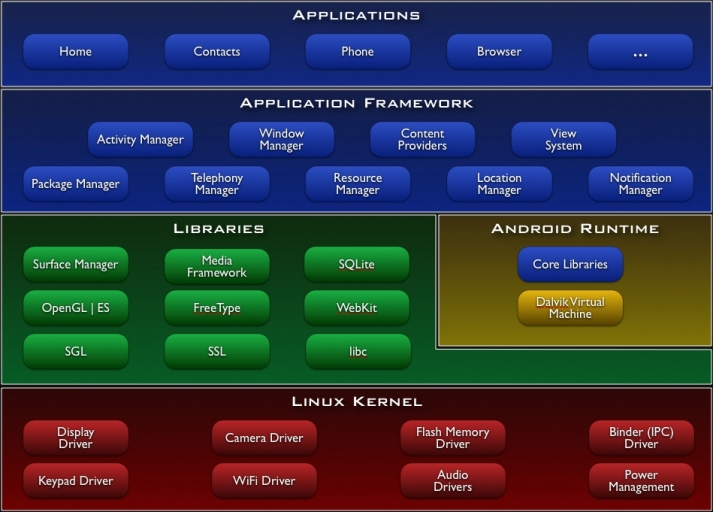
\includegraphics[width=10cm]{img/system-architecture.jpg}
    \caption{Arquitetura da plataforma Android}
    \label{system-architecture}
\end{figure}

\subsubsection{Application}
Android será distribuido com um conjuto de aplicações centrais, incluindo um cliente
de e-mail, programa de SMS, calendário, mapas, navegador, entre outros. Todas as 
aplicações são escritas em Java.

\subsubsection{Application Framework}
Fornecendo uma plataforma de desenvolvimento aberta, Android permite aos desenvolvedores
criarem aplicações extremamente ricas e inovadores. Desenvolvedores são livres para
tirar vantagem do hardware dos dispositivos, acessar informações de localização, 
executar serviços em backgrounds, definir alarmes e notificações para a barra de 
status etc.

Desenvolvedores tem total acesso às mesmas API's do framework usadas pelas aplicações 
do núcleo. A arquitetura da aplicação é projetada para simplificar o reuso de componentes;
qualquer aplicação pode publicar suas capacidades(?) e qualquer outra aplicação pode 
fazer uso dessas capacidades (sujeito às restrições de segurança impostas pelo 
framwork). Esse mesmo mecanismo permite que componentes sejam substituídos pelo 
usuário.

Os principais componentes do Application Framework são:
\begin{itemize}
\sloppy % evita que em linhas muito longas o espaço entre as palavras seja
        % aumentado
    \item System View: uma 'view' representa um widget que aparece na tela
    \item Content Providers: permite que aplicações possam acessar dados de outras 
    aplicações, ou compartilhar seus dados com outras
    \item Resource Manager: fornece acesso para recursos que não são código, como 
    strings de localização, gráficos e arquivos de layout
    \item Notification Manager: permite que as aplicações exibam alertas customizados 
    na barra de status
    \item Activity Manager: gerencia o ciclo de vida das aplicações e fornece um 
    mecanismo comum de navegação
\fussy % dual do \sloppy
\end{itemize}

\subsubsection{Libraries}
Android inclui um conjunto de bibliotecas C/C++ usada por vários componentes do 
sistema. Esses recursos são expostos para os desenvolvedores através do "application 
framework". Algumas das principais bibliotecas são listadas a seguir:

\begin{itemize}
    \item System C library - implementação da bibliotec padrão C (libc), otimizado
    para dispositivos embarcados baseados em Linux
    \item Media Libraries - as bibliotecas suportam a maioria dos formatos mais 
    populares de audio, video e imagem, incluindo MPEG4, H.264, MP3, AAC, AMR, 
    JPG, e PNG
    \item Surface Manager - gerencia o acesso o subsistema do display e composição 
    suave de camadas 2D e 3D para múltiplos dispositivos
    \item LibWebCore - um moderno mecanismo para navegador web que possibilita tanto o 
    navegador do Android quanto um visualizador web embutido
    \item SGL - o mecanismo para gráficos 2D subjacente
    \item 3D libraries - uma implementação baseada na API OpenGL ES 1.0; as bibliotecas
    podem tanto usar a aceleração 3D por hardware (quando disponível), quanto
    a renderação 3D otimizada por software, já incluida.
    \item FreeType - renderização de fonte vetorial e bitmap
    \item SQLite - um poderoso e leve mecanismos de banco de dados relacional, 
    disponível para todas as apliações
\end{itemize}

\subsubsection{Android Runtime}

Android inclui um conjunto de biblitocas básicas que provê a maioria das funcionalidades
disponíveis na biblioteca padrão da linguagem de programação Java.

Cada aplicação Android executa em seu próprio processo, com sua própria instância 
da máquina virtual Dalvik. Dalvik foi escrita de forma a permitir que um dispositivo
execute multiplas MV's eficientemente. A MV Dalvik executa arquivos no formato de 
Executáveis Dalvik (.dex) que é otimizado para usar o mínimo de memória possível. 
A MV é baseado em registradores, e executa classes compiladas por um compilador Java 
que transforma essas classes no formato .dex com a ferramenta "dx".

\subsubsection{Linux Kernel}

Android depende da versão 2.6 do Linux para serviços do núcleo do sistema como 
segurança, gerência de memória, gerência de processos, pilha de rede e modelo de 
drivers. O núcleo também atua como uma camada abstrata entre o hardware e o resto
da pilha de sofware.

\subsection{Arquitetura de aplicações Android}

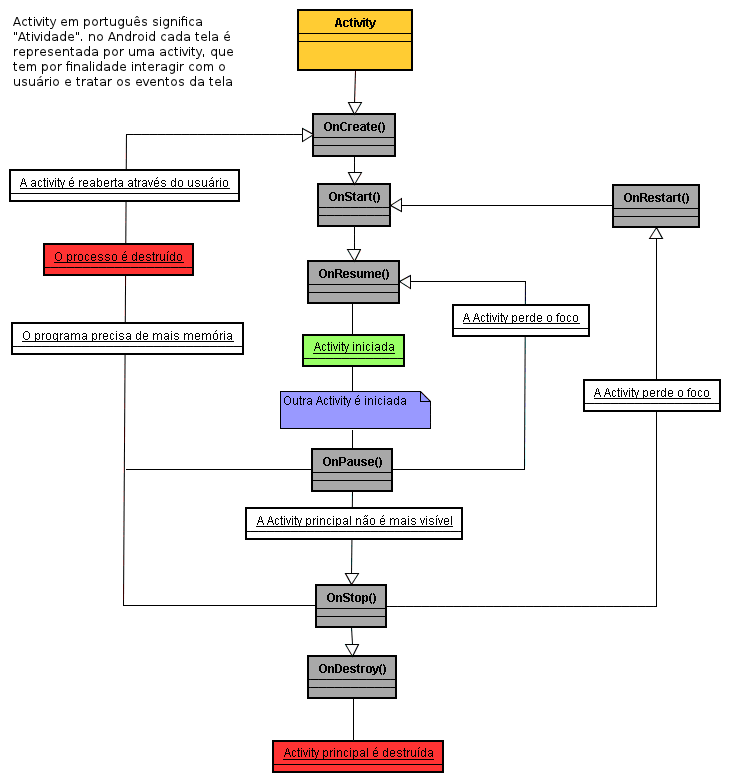
\includegraphics[width=10cm]{img/Activity_lifecycle}

\begin{itemize}
    \item Não existe método main()
    \item Uma aplicação pode ter quatro tipos de componentes:
    \item Activity: interfaces com o usuário (tela)
    \item Service: executa em background, sem interface com o usuário
    \item Broadcast receivers: apenas recebe e reage a mensagens de broadcast
    \item Content providers: compartilhar dados da aplicações com outras aplicações
\end{itemize}

% ------------------------------------------------------------------------------
\section{Estudo de caso: Froid - Fortunes for Android}

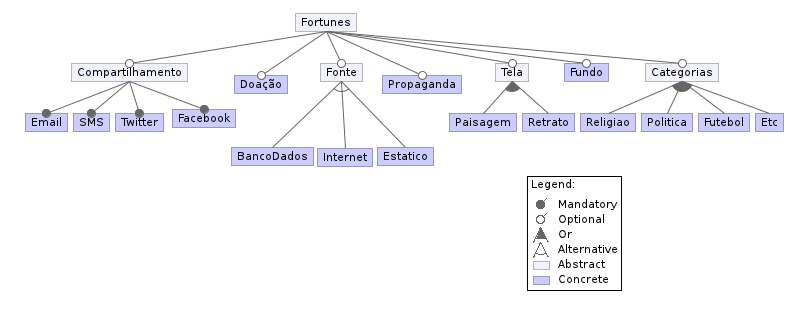
\includegraphics[width=10cm]{img/fortunes_fm}

% ..............................................................................
\section{Pontos de variações em dispositivos com Android}

\begin{itemize}
    \item Versão da API
    \item Dispositivos com ou sem sensores
    \item Gráficos 2D ou 3D
    \item Mecanismo de interação
    \item Pacote de compatibilidade
    \item Versão da OpenGL ES
    \item Android NDK           
    \item Tamanhos e densidade das telas
    \item Línguas internacionais
\end{itemize}

% ..............................................................................
\section{Mecanismos de controle de variabilidades}
\begin{itemize}
    \item  Polimorfismo
    \item Reflexão
    \item Classe wrapper
    \item Checagens de versão da API e de recursos do aparelho em tempo de execução
    \item Atributos final e Compilação Condicional 
    \item Recursos da Aplicação
\end{itemize}

% ..............................................................................
\subsection{Polimofirmo}
No Froid, o controle das variabilidades para a Fonte das fortunes é feita através 
da implementação da interface FortuneProvider.

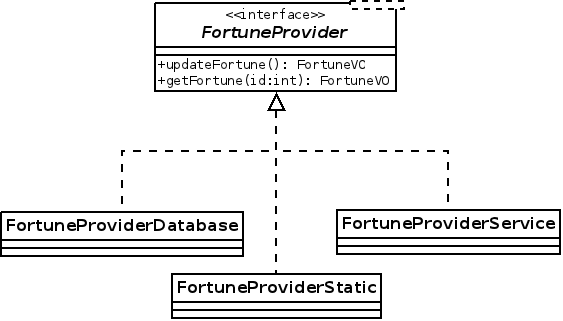
\includegraphics[width=10cm]{img/implementacao_FortuneProvider}
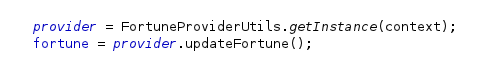
\includegraphics[width=10cm]{img/instaciando_provider}
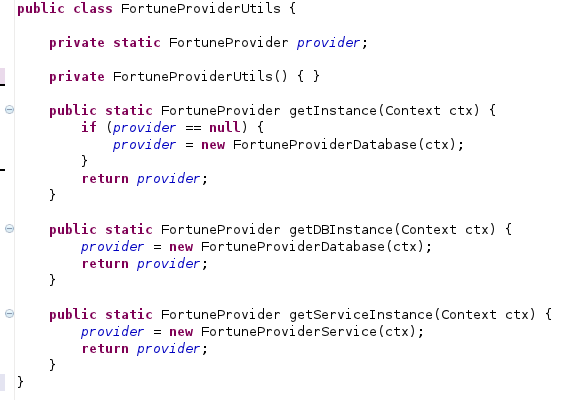
\includegraphics[width=10cm]{img/FortuneProviderUtils}
% ------------------------------------------------------------------------------
\subsection{Reflexão}

Texto + imagens do slide 22

% ..............................................................................
\subsection{Classe wrapper}

Texto + imagens dos slides 23-25

% ..............................................................................
\subsection{Checagem da versão em tempo de execução}

Texto + imagens dos slides 26

% ..............................................................................
\subsection{Checagem da existência de um determinado recurso}
Pode-se utilizar o método PackageManager.hasSystemFeature() para determinar se o 
dispositivo possi um determinado recurso

% ..............................................................................
\subsection{Atributos com modificadores final}

Texto + imagens dos slides 28


% ..............................................................................
\subsection{Compilação condicional}

Texto + imagens do slide 29


% ..............................................................................
\subsection{Recursos da aplicação}

Texto + imagens dos slides 30-34


% ..............................................................................
\subsection{Compartilhamento de informações}

Texto + imagens dos slides 25


% ==============================================================================
\chapter{Conclusão}

% ..............................................................................
\section{Pré-avaliação}
Em se tratando de gerência da variabilidades, há todo um campo de estudo pela 
frente \\
Com os mecanismos atuais, as aplicações ficarão inchadas

% ------------------------------------------------------------------------------
\section{Trabalhos futuros}
 Implementar ou estudar uma LPS de fato para o Android 

% ==============================================================================
\nocite*
\bibliographystyle{apalike}
%\bibliographystyle{abnt-alf}
\bibliography{biblio}

% ==============================================================================
\end{document}
